\chapter{The Standard Model of Particle Physics}
\label{chap:sm}

The objects responsible for chemistry are found in the periodic table of the elements seen in Figure \ref{fig:periodictable}. Quantum mechanics was developed in the early 20th century and gave an explanation for the experimentally determined structure to the period table of elements.
\begin{figure}[htbp]
\centering
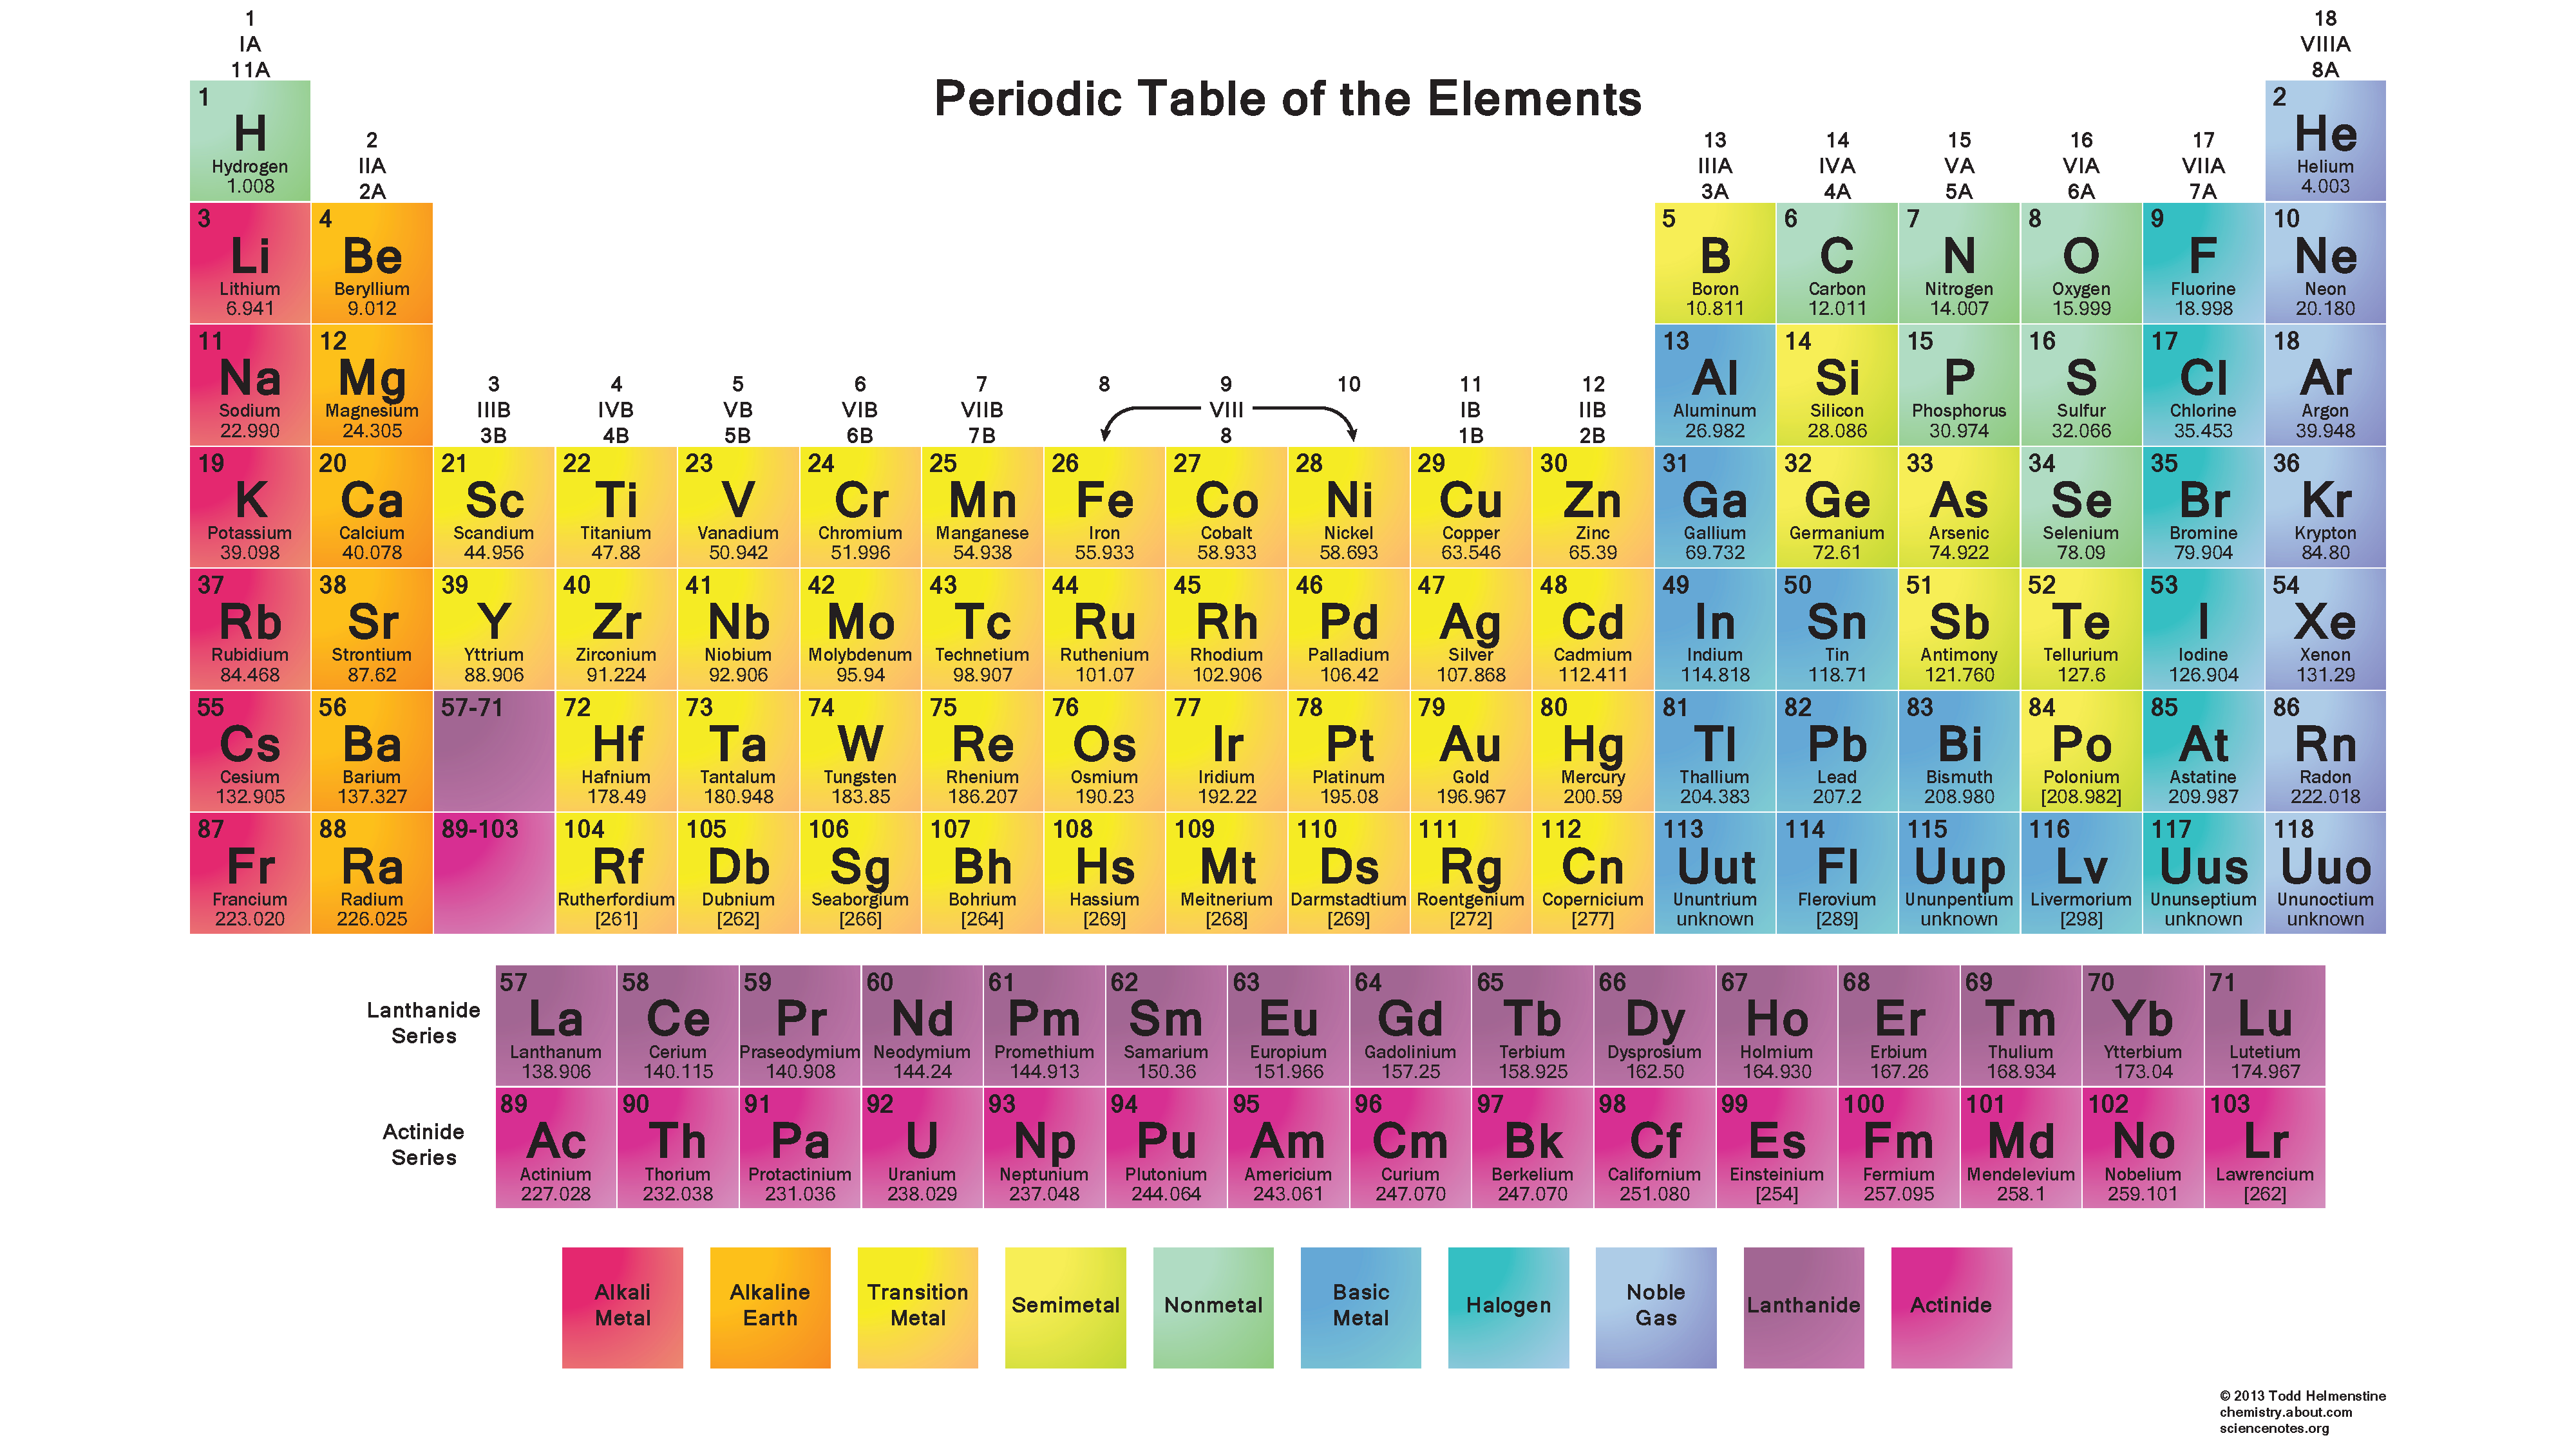
\includegraphics[width=0.85\textwidth]{figs/PeriodicTable.pdf}
\caption{The periodic table of elements.}
\label{fig:periodictable}
\end{figure}

But the elements themselves are made of more fundamental ``atoms'' described by the Standard Model of particle physics, the current knowledge is summarized in another table, seen in Figure \ref{fig:sm}.

The discovery of the Higgs (H) boson in 2012 was a monumental achievement solidifying the SM as it found the final fundamental particle within the theory.\cite{201230} 

\begin{figure}[htbp]
\centering
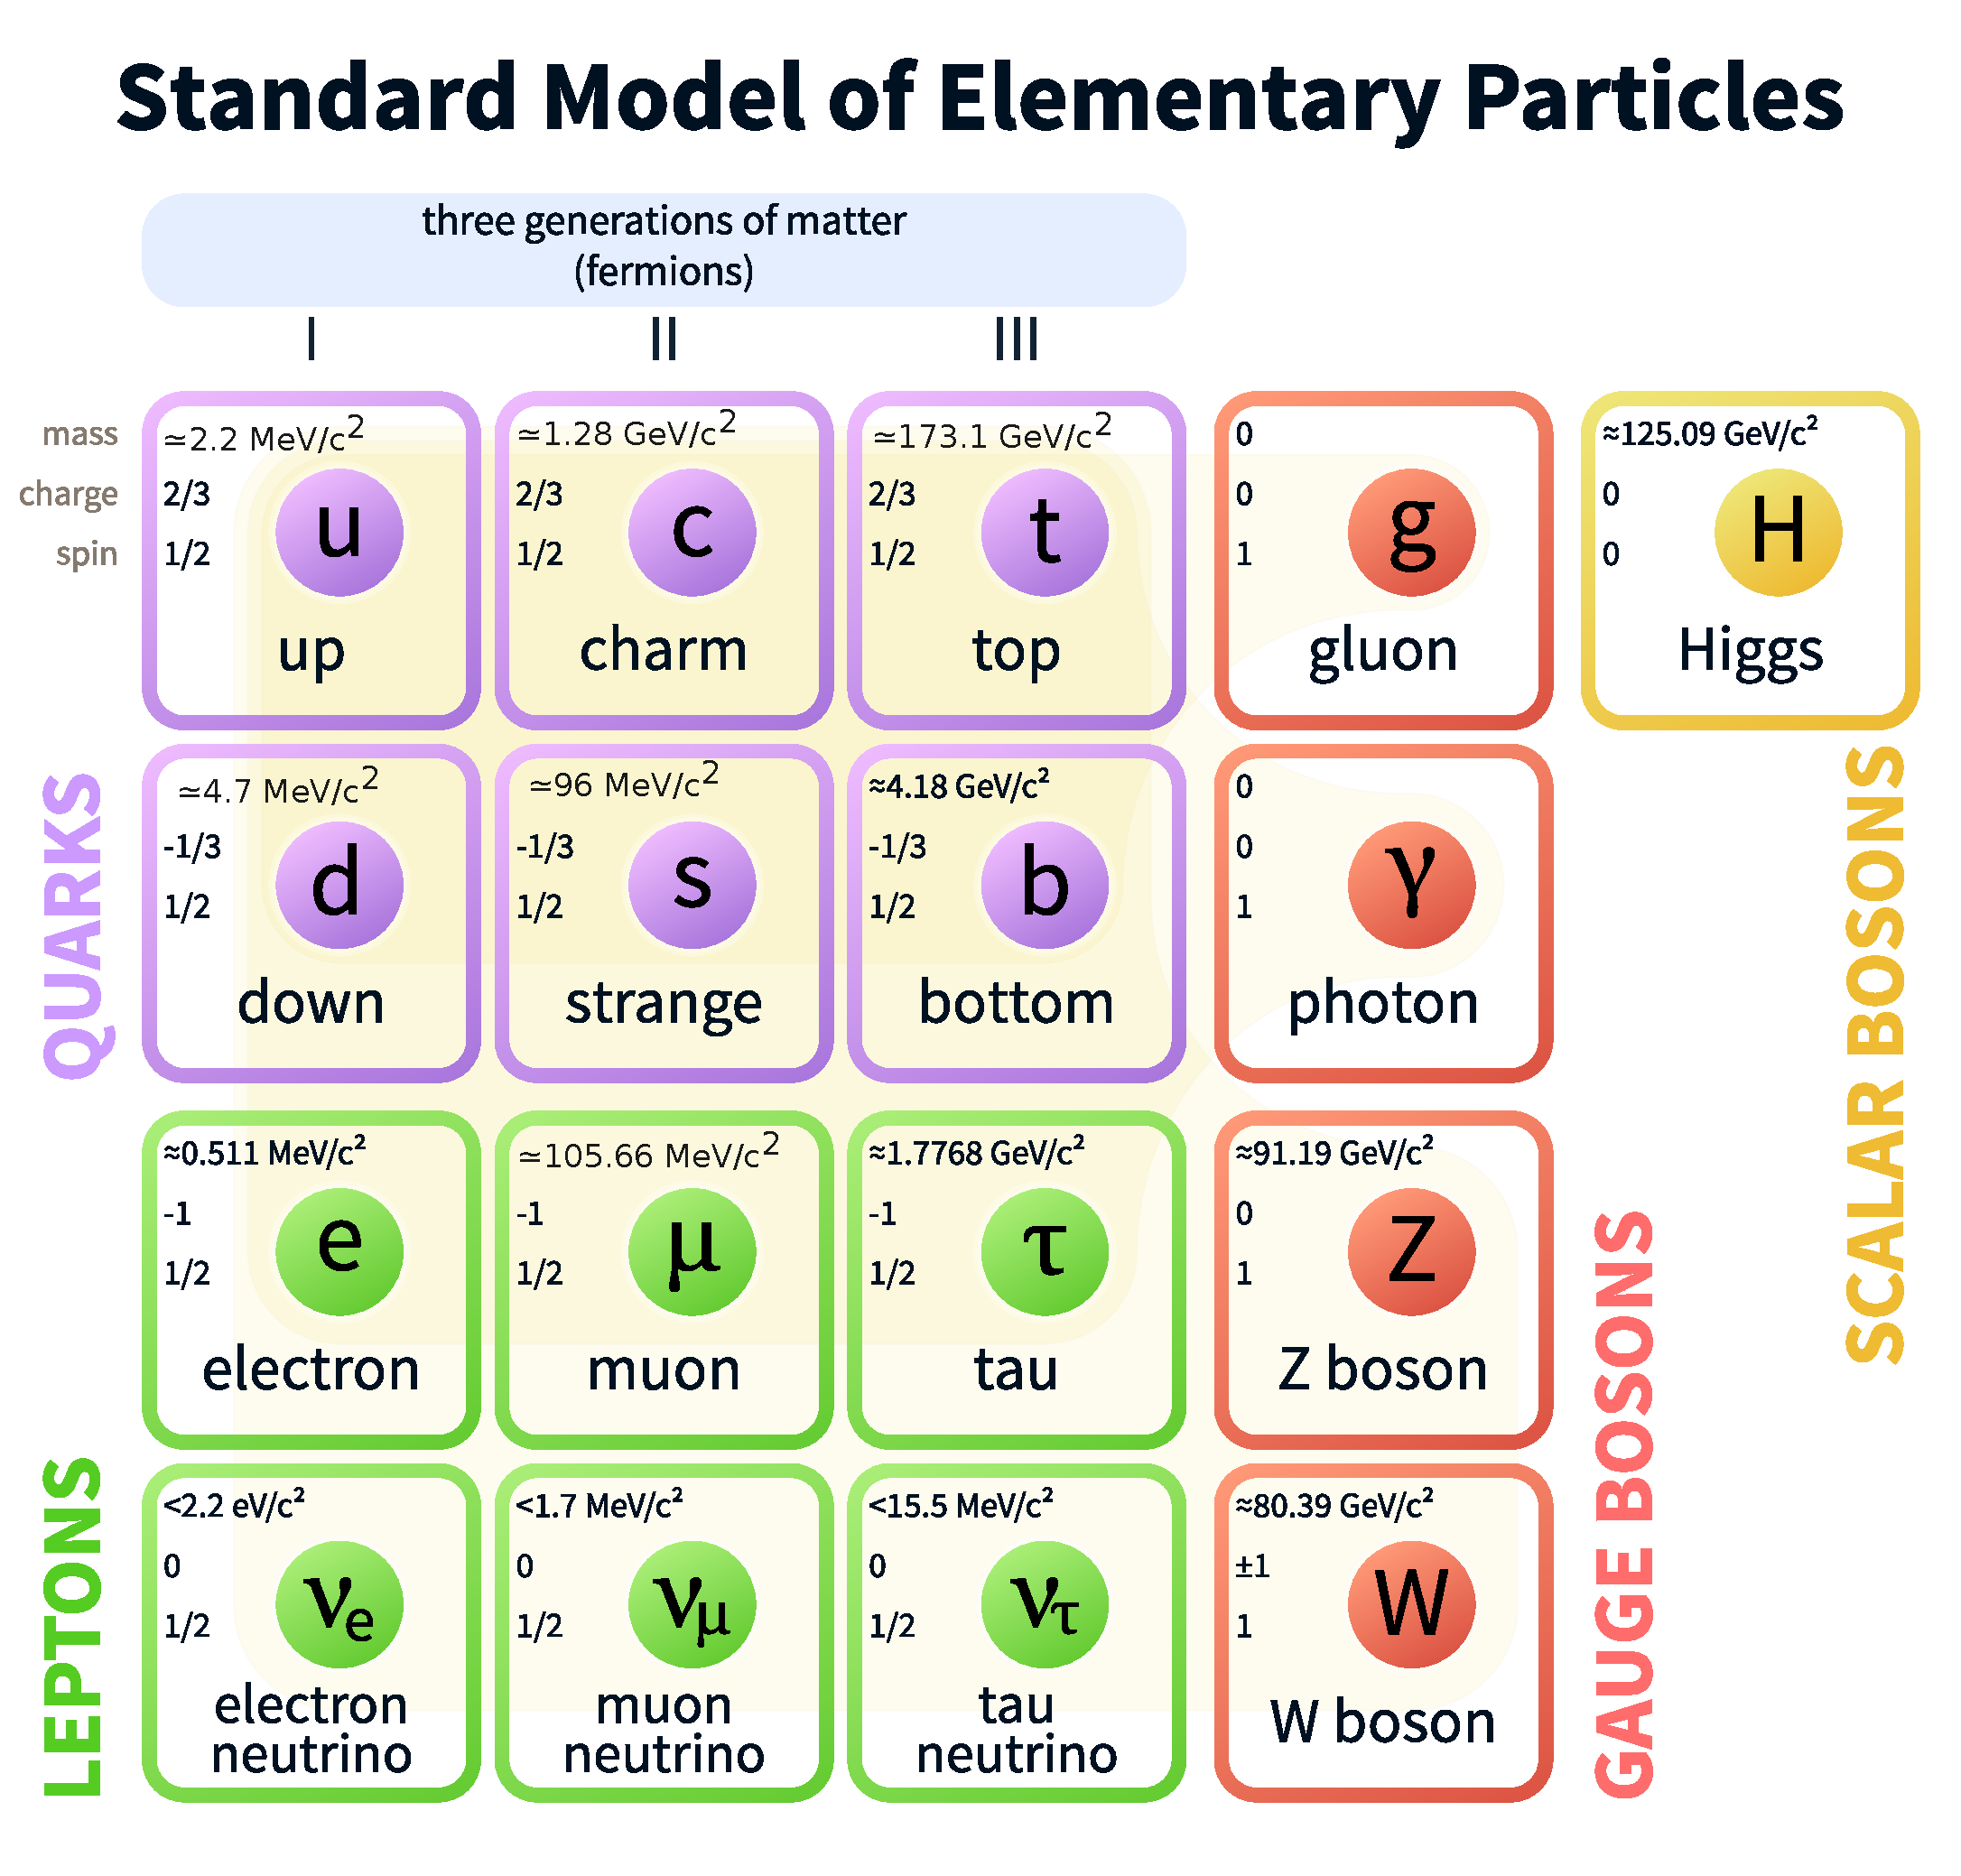
\includegraphics[width=0.7\textwidth]{figs/StandardModelofElementaryParticles.pdf}
\caption{The particles of the Standard Model.}
\label{fig:sm}
\end{figure}

\section{Electroweak}
\section{Spontaneous Symmetry Breaking}
\section{Quantum Chromodynamics}
\section{Supersymmetry}
